\chapterimage{./Pictures/cover-socket} % Chapter heading image
\chapter{TP7+TP8 : Communication socket}

\section{Communication distante en utilisant l’outil netcat}

\subsection{Exercice 1 : Découverte de la commande nc : netcat}
\textit{L’objectif de cet exercice est de nous familiariser avec une commande puissante appelée \mintinline{shell}{nc}. Cette commande, inspirée de la commande \mintinline{shell}{cat}, permet d’afficher et de recevoir un flux d’octets, non pas à l’écran et depuis le clavier, mais sur ou depuis le réseau, et plus précisément vers un processus distant identifié par une adresse ip un numéro de port et un mode (connecté "TCP" ou non connecté "UDP")}

\subsection{Exercice 2 : Utilisation de la commande nc : netcat pour le transfert de fichier et l’évaluation de la bande passante}
\textit{La commande netcat, souvent réduite au nom nc, est un utilitaire très puissant qui reprend le principe de la commande cat sur un support réseau. Les possibilités de cette commande sont énormes, et permettent de mettre en place très simplement un serveur en mode connecté ou non connecté pour transférer du texte ou un fichier. Cette commande peut également jouer le rôle de client.}

\subsection{Exercice 3 : Une histoire de serveurs concurrents ...}
\textit{Dans cet exercice, nous regardons quelles capacités de cohabitation existent entre des serveurs qui voudraient utiliser le même port de communication}

\subsection{Exercice 4 : Comprendre une requête HTTP}
\textit{Dans cet exercice, nous regardons une utilisation simple et originale de \mintinline{shell}{netcat} : comprendre ce que votre navigateur internet envoie comme information lorsqu’il effectue une requête sur un site web}

\section{Développement d’un client et d’un serveur en C}

\subsection{Exercice 5 : Mise en place d’une communication en mode non connecte}
\textit{L’objectif de cet exercice est de découvrir les fonctions et structures de base en C permettant une communication en mode non connecté UDP.}
Nous proposerons le code ci-dessous afin d'implementer un client UDP ayant le comportement demandé :
\inputminted[linenos,firstline=31, lastline=87]{cpp}{../sources/cpp/TP7-8/clientUDP.c}

Nous proposerons le code ci-dessous afin d'implementer un serveur UDP ayant le comportement demandé :
\inputminted[linenos,firstline=34, lastline=104]{cpp}{../sources/cpp/TP7-8/serveurUDP.c}

Après avoir lancé le serveur UDP nous testerons la communication entre le serveur UDP et le client UDP à l'aide de la commande \mintinline{bash}{UDClient <IP> <port> <message>} ainsi nous précisons au client l'IP et le port du serveur mais aussi le message que nous souhaitons envoyer.
\mintinline{shell}{0.0.0.0 5000 "tset ysae"}

\subsection{Exercice 6 : Création d’une architecture (client UDP) - (relai UDP-TCP) - (serveur TCP)}
\textit{L'objectif de cet exercice est de manipuler les deux mode (connecté et non connecté), en faisant communiquer un serveur tournant en TCP avec un client tournant en UDP. Cette communication n’est pas directement possible et nécessite un processus intermédiaire qui fera le relai entre le client et serveur.}

\begin{figure}[H]
\centering
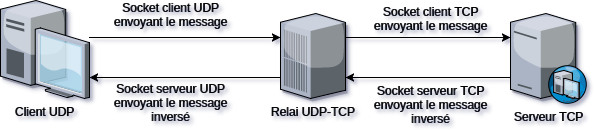
\includegraphics[width=300pt]{./cpp/Pictures/tp7+tp8-relay-UDP-TCP}
\caption{Relai UDP-TCP}
\label{Relai UDP-TCP}
\end{figure}

À l'aide des instructions donné dans le sujet de l'exercice nous pouvons implémenter le code principale d'un serveur TCP étant similaire à celui d'un serveur UDP.

\inputminted[linenos,firstline=34, lastline=104]{cpp}{../sources/cpp/TP7-8/serveurTCP.c}

\section{Exercices bonus}

\subsection{Exercice 7 : Résolution de noms}
\textit{Cet exercice à pour objectif de manipuler la fonction \mintinline{cpp}{gethostbyname()}. Cette fonction permet de transformer des noms de domaines en adresse ip, en interrogeant un serveur DNS.}

\begin{figure}[H]
\centering
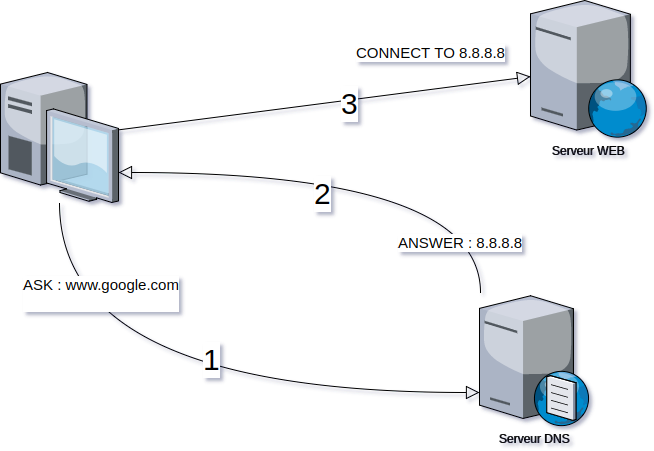
\includegraphics[width=300pt]{./cpp/Pictures/tp7+tp8-DNS}
\caption{Résolution DNS}
\label{Résolution DNS}
\end{figure}

A l’aide du manuel et des exemples disponibles sur internet, ainsi que de la documentation de la fonction \mintinline{cpp}{gethostbyname()} permettant la translation d’un nom de domaine vers une adresse IP. J'ai créé un programme qui affiche les adresses IP des noms de domaine "www.yahoo.fr", "www.gmail.com" et "www.u-bourgogne.fr".

\inputminted[linenos,firstline=10, lastline=36]{cpp}{../sources/cpp/TP7-8/getHostByName.c}

%\subsection{Exercice 8 : Serveur multi-client en mode connecté}
